% !TeX encoding = UTF-8
% !TeX spellcheck = en_GB
% !TeX root = ../thesis.tex

\chapter{Evaluation and Discussion}
\label{chapter:evaluation}
\section{Learning from the data}
    The most important finding is, that slice isolation works. That means if one slice is under a DDos attack, other slices will be unaffected. This can be seen in the following graphs:
    
    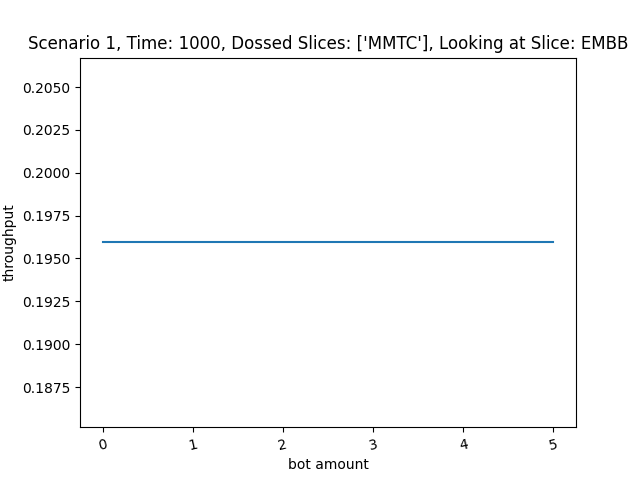
\includegraphics[width=\textwidth]{img/slice_isolation_works_single.png}
    
    This first graph shows, that the DDos attack on a slice (MMTC) has no effect on a different slice (EMBB).
    
    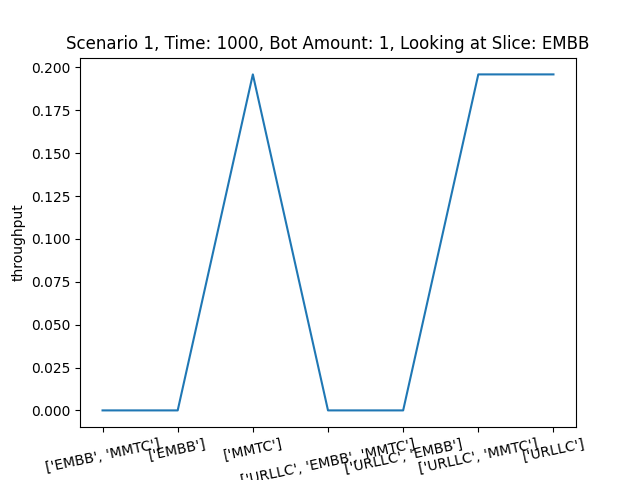
\includegraphics[width=\textwidth]{img/slice_isolation_works_dossed_slices.png}
    
    This second one shows the same point across all possible slice attacks. Only when the EMBB slice is under the attack the throughput of it decreases. This answers our second research question, that slice isolation is a useful tool as a counter measure against DDos attacks.\\
    Data evaluation can also be used in later stages from other teams. Inside our Jupyter Notebook are tools to continue the data evaluation.
    
\section{Problems with the Implementation}
    \subsection{Slicing and Machine Learning}
    Our analysis has shown that slicing prevents attacker nodes from influencing the traffic happening on other slices where no DoS-nodes are present. This enables us to isolate nodes that are executing the DDoS attack on their own slice. This way they would only influence each other.
    
    But due to our slicing implementation relying heavily on computational efforts provided by the 5G Lena network in addition to mainly using the EPSBearer for our QoS guarantees reassigning slices during runtime proved to be not possible. 
    For future implementations that aim to use machine learning for DDoS prevention via Slice Isolation it is highly recommended to use this\footnote[7]{\url{https://github.com/matteonerini/5g-network-slicing-for-wifi-networks}} WiFi-Slicing implementation as a basis for the implementation in 5G-Lena.
    
    \subsection{TCP}
    When trying to use TCP in the internet simulation no throughput could be recorded. Unfortunately we could not resolve this issue. This might be due to 5G-Lena not supporting TCP, yet, or due to our lack of understanding the network.